\documentclass[12pt, a4paper]{article}

\usepackage{amsmath}
\usepackage{array}
\usepackage{amsmath}
\usepackage[portuguese]{babel}
\usepackage{chngpage}
\usepackage{float}
\usepackage[a4paper, margin=2cm]{geometry}
\usepackage{graphicx}
\usepackage{hyperref}
\usepackage{listings}
\usepackage{setspace}
\usepackage{xcolor}

\lstdefinestyle{codestyle}{
    commentstyle=\color{teal},
    keywordstyle=\color{blue},
    numberstyle=\ttfamily\color{gray},
    stringstyle=\color{red},
    basicstyle=\ttfamily\footnotesize,
    breakatwhitespace=false,
    breaklines=false,
    keepspaces=true,
    numbers=none,
    showspaces=false,
    showstringspaces=false,
    showtabs=false,
    tabsize=4
}
\lstset{style=codestyle}

\title{\Huge \textbf{Análise e Testes de Software \\ \Large Trabalho Prático}}
\date{4 de junho 2025}

\begin{document}

\begin{center}
    \includegraphics[width=0.25\textwidth]{res/cover/EE-C.eps}
\end{center}

\chardef\_=`_
\onehalfspacing
\setlength{\parskip}{\baselineskip}
\setlength{\parindent}{0pt}
\def\arraystretch{1.5}

{\let\newpage\relax\maketitle}
\maketitle
\thispagestyle{empty}

\vspace{\fill}

\begin{adjustwidth}{-2cm}{-2cm} % These values only need to be large enough to center the table
    \begin{center}
        \begin{tabular}{>{\centering}p{0.25\textwidth}
                        >{\centering}p{0.25\textwidth}
                        >{\centering\arraybackslash}p{0.25\textwidth}}

            Humberto Gomes & José Lopes & Mariana Cristino \\
            A104348        & A104541    & A90817
        \end{tabular}
    \end{center}
\end{adjustwidth}

\pagebreak

\begin{abstract}
    Neste projeto de Análise e Testes de \emph{Software}, foram utilizadas diversas técnicas para
    encontrar falhas numa aplicação Java. Em primeiro lugar, utilizando \emph{white-box testing},
    foram escritos testes unitários para os diversos subsistemas da aplicação, cuja cobertura
    (\emph{branch} e \emph{mutant coverage}) foi analisada. Também foram utilizadas diversas
    metodologias para geração automática de casos de teste, como o EvoSuite, um sistema construído à
    mão com recurso ao QuickCheck, e LLMs, cuja cobertura dos resultados também foi analisada. Em
    relação aos resultados obtidos, concluiu-se que os testes unitários, apesar de serem os que
    mais exigem recursos humanos, foram os mais capazes de encontrar falhas no código.
\end{abstract}

\section{Gradle}

Para automatizar a compilação e testagem deste projeto, foi utilizado o Gradle. No Gradle, a
definição de um projeto é feito de forma imperativa, enquanto que no Maven, a ferramenta utilizada
nas aulas práticas, é feita de forma declarativa. Deste modo, foi possível implementar diversas
funcionalidades no sistema de compilação que teriam sido consideravelmente mais difíceis (ou até
impossíveis) de implementar em Maven.

Em primeiro lugar, o projeto suporta todas as tarefas comuns de um projeto Java, como \texttt{run},
\texttt{build}, \texttt{test}, \texttt{jar}, \emph{etc.}. No entanto, estas tarefas foram estendidas
para suportarem mais funcionalidades, sendo as maiores mudanças as da tarefa \texttt{test}. Uma
destas mudanças foi a medição automática de cobertura de código, feita com o JaCoCo. Ademais, foi
adicionado suporte para mais do que uma \emph{suite} de testes, para ser possível fazer comparações
entre a qualidade dos diversos tipos de teste utilizados (testes unitários ou gerados
automaticamente). Para trocar de \emph{suite} de testes, a propriedade \texttt{testDir} deve ser
utilizada, como mostra o exemplo abaixo:

\begin{center}
    \texttt{gradle test -PtestDir=oldunittests}
\end{center}

Outra funcionalidade implementada foi a asserção da versão utilizada do Java conforme a tarefa a
ser executada. Por exemplo, na geração e execução de testes EvoSuite, o Gradle foi programado para
apenas aceitar a versão 8 do JDK, enquanto que a versão 21 deve ser utilizada para as restantes
tarefas. Também durante a execução de testes EvoSuite, o Gradle foi programado para automaticamente
utilizar o JUnit 4, em vez do JUnit 5.

Muitas tarefas implementadas no Gradle servem para interagir com o projeto Cabal utilizado para
geração de testes com o QuickCheck: o Gradle faz \emph{pass-through} de alguns comandos, garantindo
antes que as dependências de cada tarefa foram executadas. Por exemplo, para gerar os teste
unitários, é necessário que o projeto Java seja compilado em primeiro lugar, e o Gradle é
responsável por garantir que isso acontece.

Por último, também foram implementas outras tarefas, para uso do PIT e para formatação automática
de código (feita com recurso ao \texttt{clang-format}). Segue-se uma lista das tarefas mais
importantes:

\begin{itemize}
    \item \texttt{gradle build}              -- Compilar os projetos Java e Haskell
    \item \texttt{gradle run}                -- Executar a aplicação Java (\texttt{MakeItFit})
    \item \texttt{gradle test -PtestDir=...} -- Executar uma \emph{suite} de testes JUnit
    \item \texttt{gradle pit}                -- Executar o PIT para \emph{mutation testing}
    \item \texttt{gradle format}             -- Formatar o código Java e Haskell
    \vspace{1cm}
    \item \texttt{gradle generateQuickCheckTests}    -- Gerar testes com o QuickCheck
    \item \texttt{gradle generateEvoSuiteCheckTests} -- Gerar testes com o EvoSuite
    \vspace{1cm}
    \item \texttt{gradle repl}    -- Execução do GHCi no projeto Haskell
    \item \texttt{gradle haddock} -- Geração de documentação para o projeto Haskell
\end{itemize}

O Gradle, apesar da sua curva de aprendizagem acentuada, provou-se extremamente capaz de lidar com
um projeto complexo, que envolvia o uso de diversas ferramentas, várias versões de Java, e duas
linguagens de programação.

\section{Testes Unitários}

Para o desenvolvimento de testes unitários, utilizou-se \emph{white-box} testing, ou seja, o código
fonte a ser testado foi utilizado na criação dos testes unitários. Estes testes utilizam o
\emph{runtime} do JUnit 5 para execução automática e suporte para asserções.

\subsection{Utilizadores}

No subsistema dos utilizadores, os testes unitários revelaram várias falhas no código. Uma das mais
relevantes é a incorreção na implementação dos métodos \texttt{equals}:

\begin{lstlisting}

if (o == this)
    return true;
if (this instanceof User)
    return false;

User u = (User) o;
return ...
\end{lstlisting}

Como se pode calcular, quando se comparam dois utilizadores iguais em conteúdo mas de tipos
diferentes (ex: um utilizador amador e um profissional), o resultado obtido é o \texttt{true}. Para
corrigir este erro, o segundo \emph{if-statement} foi substituído pelos seguintes:

\begin{lstlisting}

if (o == null)
    return false;
if (this.getClass() != o.getClass())
    return false;
\end{lstlisting}

Também foi encontrado um erro em que o método \texttt{addActivities} da classe \texttt{User} violava
o encapsulamento. No entanto, a maioria dos erros encontrados tratavam-se de violações do princípio
SLAP (\emph{Single Layer of Abstraction Principle}). Por exemplo, a class \texttt{User} não validava
os valores passados nos construtores e nos \emph{setters}, sendo esta validação feita pelo
\texttt{UserManager}, uma \emph{facade} do subsistema. Deste modo, era possível obter um utilizador,
executar um \emph{setter} com um valor inválido, e voltar a armazenar o utilizador, colocando o
sistema num estado inválido. Neste caso, foi possível melhorar a API sem quebrar o resto do
programa, mas a violação deste princípio trouxe outros problemas maiores, como a comparação
incorreta de endereços eletrónicos no \texttt{UserManager}. Os \emph{emails} devem ser comparados de
forma \emph{case-insensitive}. No entanto, devido a violações do princípio SLAP (não havia um tipo
\texttt{Email} com um método \texttt{equals} adequado), esta comparação por vezes era feita de forma
\emph{case-sensitive}, um outro erro que também foi detetado por testes e corrigido.

\subsection{\texttt{Activities}}

Durante o processo de desenvolvimento e execução de testes unitários para os componentes
relacionados às atividades físicas, foram identificadas diversas inconsistências e oportunidades de
melhoria tanto na implementação quanto na cobertura dos testes. Abaixo detalham-se os principais
pontos identificados, as correções aplicadas e a garantia de cobertura total através dos frameworks
\emph{JaCoCo} e \emph{PIT Mutation Testing}.

Na classe \texttt{Activity.java}, verificou-se a ausência do método \texttt{getSpecialization()},
necessário para garantir o contrato polimórfico com as subclasses.

Na classe \texttt{Trail.java}:
\begin{itemize}
  \item O método \texttt{setTrailType(int trailType)} não limitava corretamente os valores do tipo
  de trilho, o que foi identificado através de um \emph{mutant} que sobreviveu no PIT. Logo, foi
  realizada uma substituição da lógica condicional por:
  \begin{lstlisting}
this.trailType = Math.max(TRAIL_TYPE_EASY, Math.min(TRAIL_TYPE_HARD, trailType));
  \end{lstlisting}
  Esta abordagem assegura que \texttt{trailType} seja sempre mantido entre os limites definidos
  (\texttt{TRAIL\_TYPE\_EASY} e \texttt{TRAIL\_TYPE\_HARD}).

  \item O método \texttt{caloriesWaste()} permitia valores negativos devido a um erro aritmético,
  pois utilizava \texttt{-} onde deveria ser \texttt{+} na fórmula do cálculo de calorias. A fórmula
  foi atualizada para:
  \begin{lstlisting}
return (int) (
  (getDistance() * 0.5 + getElevationGain() * 0.1 + getElevationLoss() * 0.1)
  * index * 0.01);
  \end{lstlisting}
  Esta alteração assegura que o cálculo de calorias gastas reflita corretamente o esforço físico
  baseado nos parâmetros da atividade.
\end{itemize}

\subsection{Planos de Treino}

Na classe \texttt{TrainingPlan}, a implementação de testes unitários revelou quebras de
encapsulamento (método \texttt{getActivities}) e tipos de exceção errados. Também se descobriram
problemas que, devido a falta de documentação, não se sabe se constituem erros ou a intenção do
programador: em várias funções, é feita validação de argumentos (ex.: rejeição de valores nulos),
enquanto que noutras não é, não se sabendo se nestes últimos casos o programador se esqueceu de
uma exceção, ou se é suposto que, em caso de erro, o código falhe com uma exceção \emph{built-in} do
Java (ex.: \texttt{NullPointerException}).

Não foi possível testar a função \texttt{constructTrainingPlanByObjectives} da classe
\texttt{TrainingPlanManager} devido à sua aleatoriedade intrínseca. No entanto, esta função seria
ideal para testes baseados em propriedades, visto que o seu propósito é a geração de planos de
treino que cumprem um conjunto de condições, que dariam origem a propriedades nos testes.

\subsection{\emph{Queries}}

Durante os testes unitários realizados ao package \texttt{Queries}, foram
identificadas falhas lógicas e omissões no código original. Estas falhas foram
corrigidas, garantindo a exatidão dos resultados produzidos pelas
\emph{queries} e a cobertura total dos testes através dos \emph{frameworks}
\emph{JaCoCo} e \emph{PIT Mutation Testing}.

Na classe \texttt{HowManyAltimetryDone}, detetaram-se dois problemas principais:
\begin{itemize}
  \item No método \texttt{executeQuery} com intervalo de datas, não era
        verificado se a data da atividade se encontrava dentro do intervalo
        fornecido. Esta lógica foi acrescentada de forma a evitar contagens
        erradas de altimetria.
  \item No segundo método \texttt{executeQuery}, o cálculo da altimetria estava
        incorreto, subtraindo a perda de elevação em vez de a somar. A expressão
        foi corrigida para somar corretamente o ganho e a perda de elevação.
\end{itemize}

Na classe \texttt{MostDoneActivity}, foram feitas as seguintes correções:
\begin{itemize}
  \item Um dos ramos correspondente à atividade \texttt{Repetitions} nunca era
        executado, pois apresentava uma condição que nunca se iria verificar: a
        de existir uma atividade de tipo diferente das apresentadas. Este ramo
        foi, por isso, removido, tendo ficado apenas o \texttt{else}.
  \item O bloco \texttt{default} do \texttt{switch} representava código morto,
        pois todas as possibilidades válidas já estavam cobertas. Foi
        simplificado para refletir apenas casos efetivos e garantir a cobertura
        total dos testes.
\end{itemize}

Na classe \texttt{QueriesManager.java}, o construtor inicial recebia parâmetros
que não eram usados. Estes foram removidos para refletir corretamente a
funcionalidade da classe e evitar confusão na sua utilização.

\subsection{Utilitários}

Durante a execução dos testes unitários ao \emph{package} \texttt{Utils}, foi
identificado um problema relevante na classe \texttt{EmailValidator.java},
responsável por validar endereços de correio eletrónico.

O padrão original utilizado para a validação de emails era demasiado restritivo
e falhava em reconhecer múltiplos endereços válidos de acordo com a
especificação RFC. Esta limitação resultava em várias falhas nos testes,
nomeadamente com emails com carateres especiais ou domínios válidos menos comuns.

Para resolver esta situação, o padrão original:
\begin{verbatim}
"^[a-zA-Z0-9.+_-]+@[a-zA-Z0-9.-]+\\.[a-zA-Z]{2,}$"
\end{verbatim}
foi substituído por uma expressão regular mais abrangente que, ainda que não
atenda a todos os padrões RFC, é mais competente que a anterior, e permite
uma maior correção na hora de avaliar endereços eletrónicos.
\subsection{\texttt{MakeItFit}}

Diversos métodos de atualização de atributos do utilizador estavam incorretamente a chamar
\texttt{this.userManager.updateUser(user)}, mesmo não sendo necessária tal invocação devido ao
padrão de agregação usado (e não composição). Foram aplicadas as seguintes correções:

Métodos corrigidos:
\begin{itemize}
    \item \texttt{updateUserName}
    \item \texttt{updateUserAge}
    \item \texttt{updateUserWeight}
    \item \texttt{updateUserHeight}
    \item \texttt{updateUserBpm}
    \item \texttt{updateUserLevel}
    \item \texttt{updateUserPhone}
\end{itemize}

Foi removida a chamada de \texttt{updateUser(user)}, pois as alterações ao objeto \texttt{User} são
refletidas automaticamente devido à agregação.

No método \texttt{updateUserEmail}, o caso é diferente, pois altera a chave identificadora do
utilizador (o email). De modo que, a chamada de \texttt{updateUser(user)} foi substituída por:
\begin{verbatim}
    this.userManager.removeUserByEmail(email);
    this.userManager.insertUser(user);
\end{verbatim}

Este erros foram detetados, devido ao desenvolvimento de testes unitários robustos que asseguram a
cobertura total do código.

Os testes cobrem condições normais, limites, entradas inválidas e casos extremos, garantindo assim
confiabilidade e robustez no comportamento das funcionalidades relacionadas às atividades e à gestão
de utilizadores.

\subsection{Resultados Obtidos}

Para os testes unitários desenvolvidos, apresentam-se as coberturas medidas abaixo:

\begin{figure}[H]
    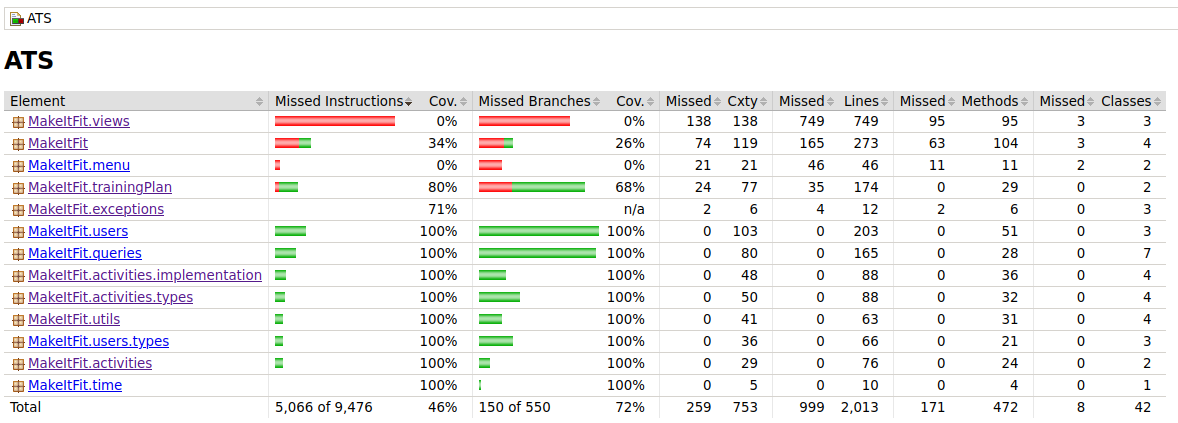
\includegraphics[width=\textwidth]{res/Jacoco.png}
    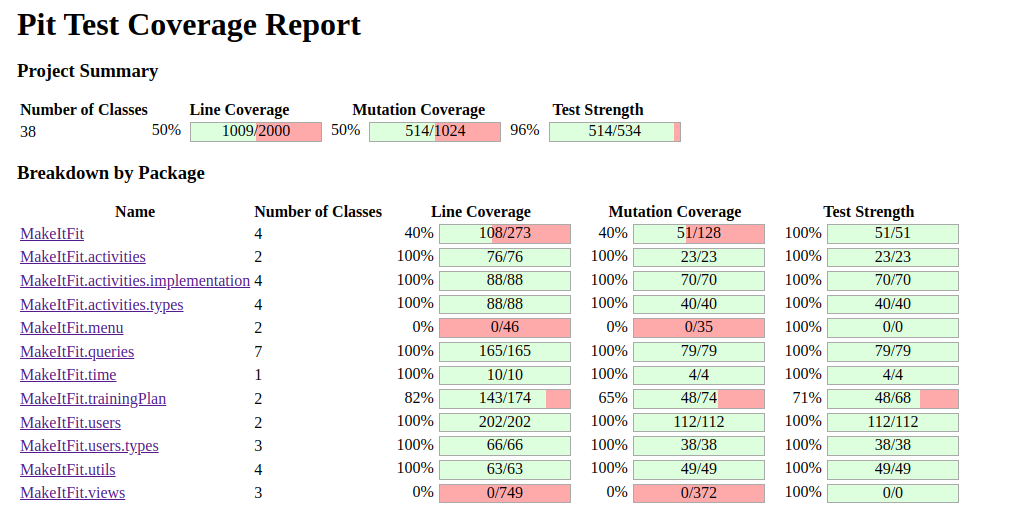
\includegraphics[width=\textwidth]{res/Pit.png}
    \caption{Coberturas medidas com o Jacoco e com o PIT, respetivamente, nos novos testes unitários.}
\end{figure}


\section{Geração de Testes com o EvoSuite}

Para a geração de testes com o EvoSuite, foi necessário, em primeiro lugar, converter o projeto para
Java 8, visto que versões mais recentes do Java não são suportadas pelo EvoSuite. Também é
necessário que o \emph{runtime} destes testes seja executado em Java 8, pelo que não foi possível
analisar a \emph{mutation coverage} destes testes, visto que o PIT não funciona nesta versão de
Java.

Os testes do EvoSuite apresentam uma boa cobertura do código. No entanto, fazendo uma análise manual
dos mesmos, conclui-se que não são bons testes unitários em si, apesar da sua leitura poder ajudar
o desenvolvedor a encontrar erros. A título de exemplo, nos subsistemas de utilizadores e
atividades, vários testes são feitos com valores inválidos (ex.: altura negativa), o que mostra que
a validação destes valores não está a ser feita. Ademais, o EvoSuite deteta exceções que não estão
explícitas no código (ex.: \texttt{NullPointerException}), o que pode informar o desenvolvedor das
verificações que deve implementar.

Segue-se a cobertura dos testes gerados por EvoSuite:

\begin{figure}[H]
    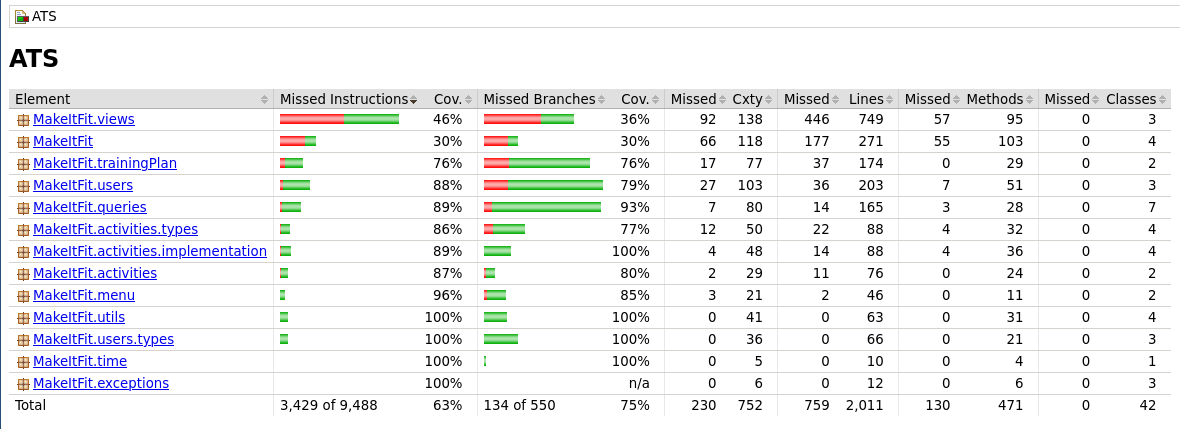
\includegraphics[width=\textwidth]{res/EvoSuiteJacoco.png}
    \caption{Cobertura medidas com o Jacoco dos unitários gerados pelo EvoSuite.}
\end{figure}

Observa-se que estas são consideravelmente superiores às da antiga \emph{suite} de testes unitários:

\begin{figure}[H]
    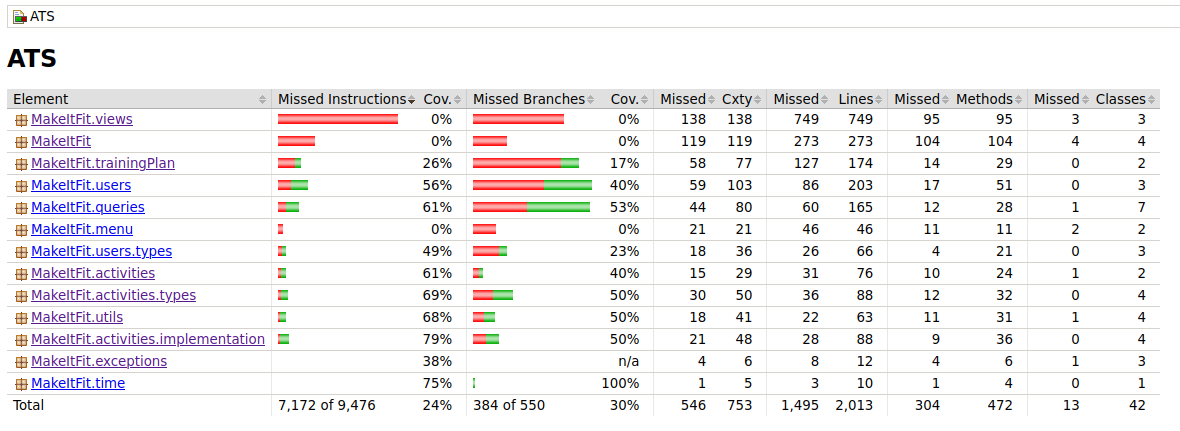
\includegraphics[width=\textwidth]{res/OldJacoco.png}
    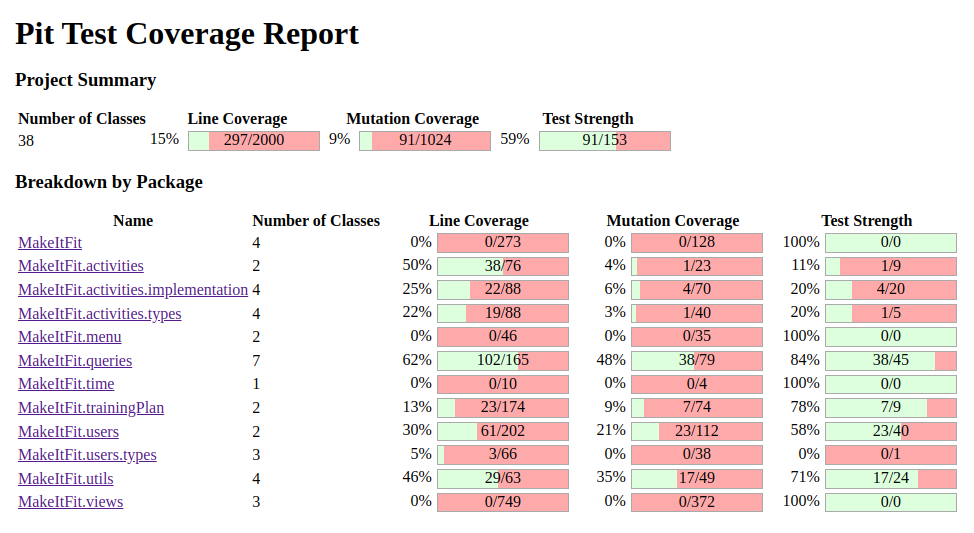
\includegraphics[width=\textwidth]{res/OldPit.png}
    \caption{Coberturas medidas com o Jacoco e com o PIT, respetivamente, nos antigos testes unitários.}
\end{figure}

\section{Geração de Testes com o QuickCheck}

\subsection{Geradores}

Para ser possível gerar casos de teste aleatórios, é necessário gerar os seus \emph{inputs}. Estes
são, frequentemente, instâncias de classes da aplicação a ser testada, pelo que foi necessário
implementar geradores para as mesmas. Foram implementados diversos geradores, com o objetivo
de criar utilizadores, atividades e planos de treino realistas. A implementação teve atenção a
vários detalhes, nomeadamente:

\begin{itemize}
  \item Geração realista de nomes: Através de uma combinação de nomes próprios e apelidos comuns em
    Portugal, foram gerados nomes plausíveis como ``José Lopes'' ou ``Humberto Silva''.

  \item Endereços completos e variados: Foram geradas moradas completas, incluindo ruas, números de
    porta, andares e cidades como ``Lisboa'', ``Porto'' e ``Braga''.

  \item Telefones válidos: Os números de telemóvel e de telefone fixo são criados com base nos
    prefixos corretos e comprimentos típicos.

  \item Emails com domínios reais: Domínios populares como \texttt{gmail.com}, \texttt{hotmail.com}
    e \texttt{yahoo.com} são utilizados, promovendo realismo, além disso, a frequência de geração de
    emails é ajustada para refletir a prevalência de cada domínio, sendo \texttt{gmail.com} o mais
    comum.

  \item Datas válidas e bem distribuídas: Foi utilizado um gerador específico para datas válidas,
      respeitando os dias de cada mês e anos entre 2001 e 2025.

  \item Valores fisiológicos credíveis: Os valores gerados para peso, altura, BPM e nível de treino
    situam-se dentro de intervalos realistas e coerentes.

  \item Frequência de treino: Utilizadores do tipo \texttt{Occasional} e \texttt{Professional}
    incluem um campo de frequência semanal, gerado com base em valores plausíveis.

  \item Atividades específicas e detalhadas: Cada tipo de atividade possui os seus próprios campos
    (ex: número de repetições e séries para \texttt{PushUp}, distância e velocidade para
    \texttt{Running}, tipo de trilho para \texttt{Trail}, entre outros).

  \item Planos de treino compostos: Foram definidos \emph{training plans} que incluem listas de
    atividades com número de repetições associado, simulando planos personalizados.
\end{itemize}

\subsection{Geração de Código}

Para simplificar a geração de testes, foi criada uma \emph{framework} simples para geração de código
Java, contendo diversas funções auxiliares para se gerar código com facilidade. Abaixo, apresenta-se
a classe \texttt{JavaData}, que pode ser utilizada para transformar um tipo de dados que a
implemente numa expressão ou variável Java:

\begin{lstlisting}

class JavaData a where
  javaTypeName :: a -> String
  toJavaExpression :: a -> String

  toJavaVariable :: String -> a -> [String]
  toJavaVariable name obj =
    [javaTypeName obj ++ " " ++ name ++ " = " ++ toJavaExpression obj ++ ";"]
\end{lstlisting}

Esta classe encontra-se implementada para os vários tipos nativos de Haskell, bem como os tipos para
os quais foram escritos geradores. Ademais, também foram implementadas outras funções utilitárias,
como \texttt{decorateTest}, que encapsula o corpo de um teste num método Java \texttt{@Test}, e
várias funções para asserções, que geram o código Java para diversas asserções JUnit 5.

\subsection{Interoperabilidade com a JVM}

Para a geração de certos testes, utilizou-se a mesma metodologia que o EvoSuite: gerar
\emph{inputs}, avaliá-los de acordo com o código Java, e finalmente colocar o resultado obtido como
valor esperado do teste. Deste modo, os testes deste tipo gerados apenas são viáveis para teste de
regressões. No entanto, são necessários para testar as partes da aplicação que não são facilmente
modeláveis em Haskell, como as diversas \emph{queries}. Afinal, não é desejado que se reimplemente o
programa dado noutra linguagem, para depois comparar as duas implementações.

Para executar código Java, procurou-se inicialmente utilizar a biblioteca JVM, que permite que
código Haskell execute \emph{statements} Java. No entanto, não se teve sucesso na sua compilação,
pelo que se adotou um método de interoperabilidade com a JVM pouco ortodoxo, porém funcional: sempre
que é necessário executar código Java, a \texttt{jshell} (um REPL para Java) é executada, os
\emph{statements} são enviados para o \texttt{stdin} do processo criado, e o \texttt{stdout} é
analisado para extrair os resultados obtidos. Este método, apesar de pouco eficiente, é possível em
qualquer distribuição Java recente, sem ser necessário o \emph{linking} com bibliotecas internas da
JVM, como seria caso as bibliotecas JVM e inline-java fossem utilizadas.

\subsection{Geração Automática de Testes}

O principal objetivo desta abordagem é automatizar a geração de código de teste em Java, assegurando
cobertura funcional das principais operações do sistema, tais como:

\begin{itemize}
  \item Obtenção de atividades associadas a um utilizador (\texttt{getActivitiesFromUser});
  \item Adição e remoção de atividades (\texttt{addActivityToUser},
  \texttt{removeActivityFromUser});
  \item Criação, obtenção, atualização e remoção de planos de treino (\texttt{createTrainingPlan},
  \texttt{getTrainingPlan}, \texttt{updateTrainingPlan}, \texttt{removeTrainingPlan});
  \item Construção de planos de treino com base em objetivos
  (\texttt{constructTrainingPlanByObjectives});
  \item Adição de atividades a planos de treino (\texttt{addActivityToTrainingPlan}).
\end{itemize}

A geração de testes é realizada por funções em Haskell que produzem listas de instruções em Java,
representando os testes a serem executados. Cada teste é encapsulado num \texttt{TestTemplate}, que
inclui:

\begin{itemize}
  \item A configuração inicial do modelo (\texttt{MakeItFit});
  \item A criação do utilizador com os seus respetivos dados e atividades;
  \item As chamadas aos métodos da API Java a serem testados;
  \item Instruções de verificação, como \texttt{assertEquals}, \texttt{assertTrue} e
  \texttt{assertThrows}.
\end{itemize}

A estrutura dos testes é parametrizada por geradores, como \texttt{Gen User} e
\texttt{Gen MakeItFitDate}, e utiliza funções auxiliares como \texttt{toJavaCreateUserArgs},
\texttt{toJavaExpression} e \texttt{assertThrows} para gerar código sintaticamente válido em Java.

Além dos testes de fluxo normal, foram gerados testes para cenários de exceção, onde se verifica se
os métodos lançam exceções apropriadas como \texttt{IllegalArgumentException} ou
\texttt{EntityDoesNotExistException}. Isto contribui para uma verificação mais rigorosa do
comportamento esperado do sistema em casos inválidos.

\subsection{Resultados Obtidos}

Seguem-se os resultados da cobertura dos testes gerados por QuickCheck:

\begin{figure}[H]
    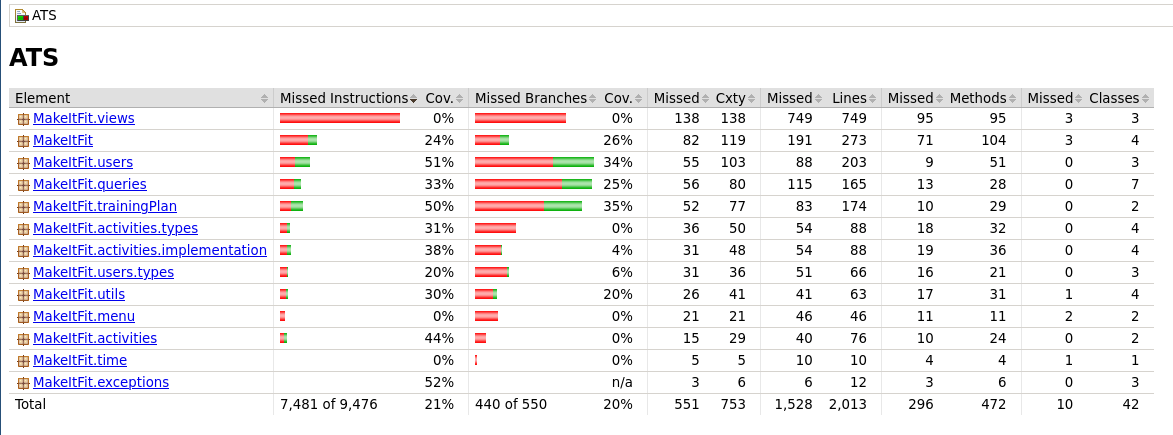
\includegraphics[width=\textwidth]{res/QuickCheckJacoco.png}
    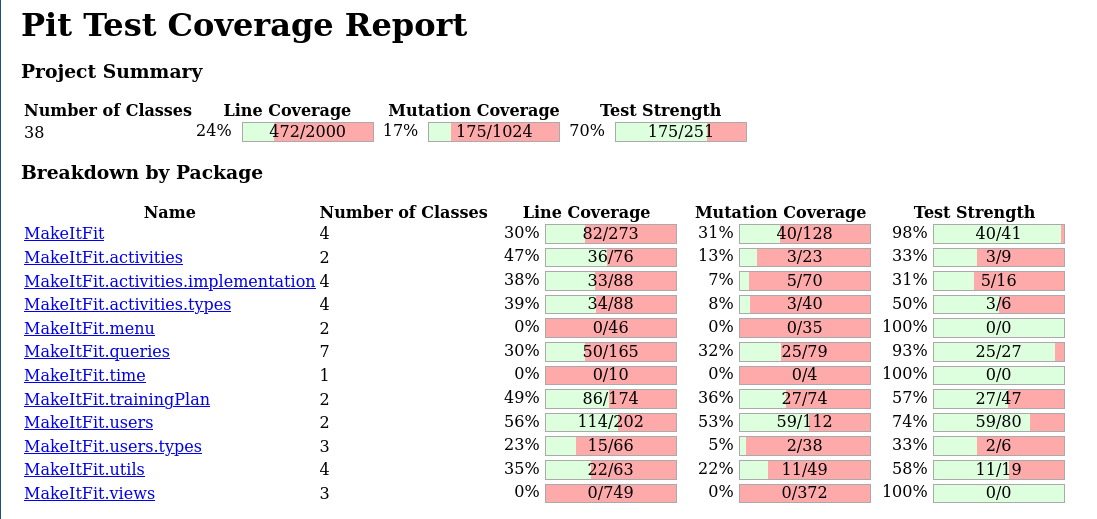
\includegraphics[width=\textwidth]{res/QuickCheckPit.png}
    \caption{Coberturas medidas com o Jacoco e com o PIT, respetivamente, nos testes gerados por QuickCheck.}
\end{figure}

\section{Testes gerados por AI}

Durante a fase de testes da aplicação \textit{MakeItFit}, foi também explorada a utilização de
inteligência artificial generativa como ferramenta de apoio à criação de testes unitários. Para este
fim, recorreu-se à IA \textit{Deepseek} treinado em grandes volumes de código-fonte aberto.

A abordagem consistiu em fornecer à IA os métodos de cada classe a serem testados. Com base nesta
informação, a IA gerou \emph{suites} de testes em Java, seguindo a API do \texttt{JUnit}. A IA
procurou inferir os casos típicos de uso, incluindo:

\begin{itemize}
  \item Criação e configuração de instâncias da classe \texttt{MakeItFit};
  \item Invocação de métodos públicos com argumentos válidos e inválidos;
  \item Utilização de instruções de verificação, como \texttt{assertEquals} e \texttt{assertThrows},
  para validar os comportamentos esperados.
\end{itemize}

A IA demonstrou competência na estruturação básica dos testes e na utilização adequada da API da
aplicação. No entanto, a sua geração baseou-se maioritariamente em inferência sem contexto profundo
do domínio da aplicação, o que resultou em testes frequentemente superficiais ou redundantes.

Apesar de gerar código funcional, a cobertura de testes obtida com a abordagem baseada em IA foi
limitada. Os testes criados cobriam sobretudo os caminhos felizes (\textit{happy paths}) e não
exploravam cenários de exceção ou combinações mais complexas de estado interno da aplicação.

Com o auxílio de ferramentas de análise de cobertura, verificou-se que os testes gerados pela
\textit{Deepseek} obtiveram uma cobertura inferior em comparação com os testes escritos manualmente.
As principais limitações observadas foram:

\begin{itemize}
  \item Ausência de testes negativos ou de fronteira;
  \item Cobertura parcial de ramos condicionais e blocos de exceção;
  \item Falta de conhecimento contextual sobre as regras de negócio da aplicação.
\end{itemize}

A utilização de IA como \textit{Deepseek-Coder} mostra-se útil para gerar testes iniciais ou esboços
de casos simples, servindo como base para desenvolvimento manual posterior. No entanto, para atingir
uma cobertura robusta e garantir a validação de cenários críticos, foi necessário complementar esta
abordagem com testes gerados por métodos mais estruturados, como o EvoSuite.

Segue-se a cobertura dos testes unitários gerados por AI:

\begin{figure}[H]
    \includegraphics[width=\textwidth]{res/AiJacoco.png}
    \includegraphics[width=\textwidth]{res/AiPit.png}
    \caption{Coberturas medidas com o Jacoco e com o PIT, respetivamente, nos unitários gerados por AI.}
\end{figure}

\section{Teste da Camada de Apresentação}

Para testar a camada de apresentação, procurou-se convertê-la para uma aplicação Web e testá-la
com Selenium. No entanto, devido a falta de tempo, apenas foi possível investigar as melhores
ferramentas possíveis para esta tarefa. Procuraram-se ferramentas que permitiriam executar código
Java num navegador Web, e encontrou-se o CheerpJ e a TeaVM. O CheerpJ, apesar da sua premissa de
executar aplicações sem qualquer alteração, não o é capaz de fazer para aplicações na linha de
comandos. Já o TeaVM exigiria ligeiras adaptações da camada de apresentação para o I/O ser feito
para uma página Web, ou seja, a implementação de um \emph{terminal emulator}. No entanto, seja qual
fosse a ferramenta utilizada, não seria possível medir a cobertura dos testes por falta de
ferramentas adequadas, pelo que também se optou por não proceder com esta solução. Uma forma mais
simples de testar a camada de apresentação da aplicação, apesar de não utilizar as ferramentas
usadas nas aulas práticas, seria a construção de \emph{strings} de entrada para a aplicação,
passadas via \texttt{stdin}, e a asserção sobre o conteúdo lido do \texttt{stdout}.

\section{Conclusão}

Neste projeto, foram aplicadas diversas metodologias de testes de \emph{software}, para procurar
detetar falhas num programa Java. Este projeto permitiu ao grupo de trabalho aprender sobre
diversas ferramentas e, de um modo mais geral, como as integrar corretamente. Em relação aos
resultados obtidos, verifica-se que, apesar de haver várias formas de gerar casos de teste de forma
automática, a qualidade destes ainda não se aproxima da de testes unitários escritos à mão, pelo
que, apesar desta metodologia ser a que mais requer recursos humanos, é que consideramos mais
adequada para a deteção de falhas num programa.

\end{document}
